\chapter{Ambiente de \textit{Data Warehousing} para Métricas de Código-Fonte}
\label{chap:arquitetura}

\section{Arquitetura do Ambiente \textit{Data Warehousing} para Métricas de Código-Fonte}
Para a implementação do ambiente de \textit{Data Warehousing} para métricas de código-fonte, foi definida a arquitetura tal como se mostra Figura \ref{arquitetura}.

\begin{figure}[ht!]
\centering
\includegraphics[keepaspectratio=false,scale=0.20]{figuras/arquitetura-dwing.eps}
\caption{Arquitetura do Ambiente de \textit{Data Warehousing} para Métricas de Código-Fonte}
\label{arquitetura}
\end{figure}
\FloatBarrier

Para selecionar as ferramentas, que implementariam cada um dos componentes, estabeleceram-se critérios gerais de seleção tal como pode ser visto na Tabela \ref{seleção}.


	\begin{table}[!ht]
	\begin{center}
	\input{tabelas/selecao.ltx}
	\caption{Critérios Gerais de seleção de ferramentas}
	\label{seleção}
	\end{center}
	\end{table}	


\section{Ferramenta de Análise Estática de Código-Fonte}

Além dos critérios gerais estabelecidos, para a escolha da ferramenta de análise estática de código-fonte, que é a fonte externa de coleta dos dados, estabeleceram-se os critérios específicos para seleção de ferramentas de análise estática de código fonte (CAE) apresentados na Tabela \ref{specific}.


	\begin{table}[!ht]
	\begin{center}
	\input{tabelas/specific.ltx}	
	\caption{Critérios Específicos para Ferramenta de Análise Estática de Código-Fonte}
	\label{specific}
	\end{center}
	\end{table}	

Após a realização de uma busca por ferramentas de análise estática de código-fonte, foram selecionados o SonarQube~\footnote{Disponível em \url{http://www.sonarqube.org/}} e o Analizo~\footnote{Disponível em \url{http:/http://analizo.org/}} cujas principais características de ambas são apresentadas na Tabela \ref{dados-ferramentas-estatica}.

\begin{savenotes}
\begin{table}[!ht]
\centering
\input{tabelas/ferramentas.ltx}
\caption{Características do SonarQube e do Analizo}
\label{dados-ferramentas-estatica}
\end{table}
\FloatBarrier
\end{savenotes}

Após levantar as características gerais de cada ferramenta, foram comparadas (SonarQube e Analizo) quanto aos critérios gerais e aos critérios específicos para ferramentas de análise estática, tal como se mostra na Tabela \ref{compare}.


\begin{table}[!ht]
\centering
\input{tabelas/compare.ltx}
\caption{Análise do SonarQube e do Analizo quanto aos critérios gerais e quanto aos critérios específicos de ferramentas de análise estática}
\label{compare}
\end{table}
\FloatBarrier

Em uma fase inicial do trabalho, fora feita a análise entre o Analizo e o SonarQube, que resultou na decisão inicial de se utilizar o SonarQube. Contudo, desde a versão 4.1, o SonarQube retirou as métricas: \textbf{LCOM4, RFC, DIT, NOC e NOM}~\footnote{CoreMetrics do SonarQube: \url{https://github.com/SonarSource/sonarqube/blob/master/sonar-plugin-api/src/main/java/org/sonar/api/measures/CoreMetrics.java}}. Dado que este fato, impacta o principal objetivo do trabalho, foi tomada a decisão de migrar para a ferramenta Analizo. Esta evoluiu e ganhou a possibilidade de emitir saídas das métricas em CSV que detalham nome da classe e as respectivas métricas, atendendo assim ao critério CAE02. Adicionalmente, o Analizo permitiu ao trabalho incorporar a análise das métricas \textbf{ANPM, AMLOC, CBO, NPA}, que como fora observado na Seção \ref{sec:clean-code}, são cruciais na detecção de cenários de limpeza de código-fonte.

\section{Projeto do \textit{Data Warehouse}}
\label{sec:project-dw}

O \textit{Data Warehouse} como elemento central do ambiente de \textit{Data Warehousing} deve ser o primeiro a ser projetado \cite{Kimball2002}. Isso ocorre, pois o DW deve ser dirigido ao negócio. Logo, a modificação do DW impacta principalmente na carga dos dados, na etapa de extração, transformação e carga, requerendo modificações conforme o DW venha a mudar.

Seguindo a metolodogia de \citeonline{Kimball2002} para o projeto de \textit{data warehouse}, apresentada na Seção \ref{sec:metodologia-dw}, foram identificados os processos de negócio e seus respectivos requisitos como se mostra nas Tabelas \ref{tab:requisitos-pecentis} e \ref{tab:requisitos-cenarios}. 


\begin{table}[H]
\centering
\input{tabelas/requisitos-percentis.ltx}
\caption{Requisitos de Negócio da Avaliação dos Valores Percentis das Métricas de Código-Fonte conforme as configurações especificadas na Tabela \ref{tab:good-metrics}}
\label{tab:requisitos-pecentis}
\end{table}
\FloatBarrier


\begin{table}[H]
\centering
\input{tabelas/requisitos-cenarios.ltx}
\caption{Requisitos de Negócio da Avaliação de Cenários de Limpeza de Código-Fonte e Avaliação de Taxa de Aproveitamento de Oportunidades de Melhoria de Código-Fonte conforme a Tabela \ref{tab:cenarios}}
\label{tab:requisitos-cenarios}
\end{table}
\FloatBarrier


Aplicando o segundo passo da metodologia de \citeonline{Kimball2002}, identificou-se a periodicidade como as \textit{releases} do software, isto é, cada software pode ter tempos diferenciados de lançamento de uma nova versão. Em alguns casos, estas podem ser semestrais ou mensais, contudo em outros casos, é possível obter \textit{releases} diárias, como resultado da integração de um determinada massa de código em um sistema de integração continua \cite{beckarticle1999}. 

Para aplicação do terceiro e quarto passo da metodologia de \citeonline{Kimball2002}, os fatos e as dimensões foram identificados a partir dos termos em negritos dos requisitos de negócio. Após a identificação dos fatos, estes foram classificados quanto à aditividade~
\footnote{\citeonline{Kimball2002} enuncia que fatos que correspondem a porcentagens e taxas são considerados não aditivos e deve-se conter, na mesma tabela, além do fato, o numerador e denominador. Este ocorre com a Taxa de Aproveitamento de Oportunidades de Melhoria de Código-Fonte} e relacionados com as respectivas dimensões conforme se mostra na Tabela \ref{tab:dimensoes-fato}.


\begin{table}[h]
\centering
\input{tabelas/dimensoes-fato.ltx}
\caption{Fatos e Dimensões do \textit{Projeto de Data Warehouse} }
\label{tab:dimensoes-fato}
\end{table}
\FloatBarrier

Tendo os fatos identificados, foram criados os diagramas de árvore, tal como proposto por \citeonline{Golfarelli1998}, tal como se vê nas Figuras \ref{fig:percentil-arvore}, \ref{fig:cenario-arvore} e \ref{fig:taxa-arvore}.

\begin{figure}[h]
\centering
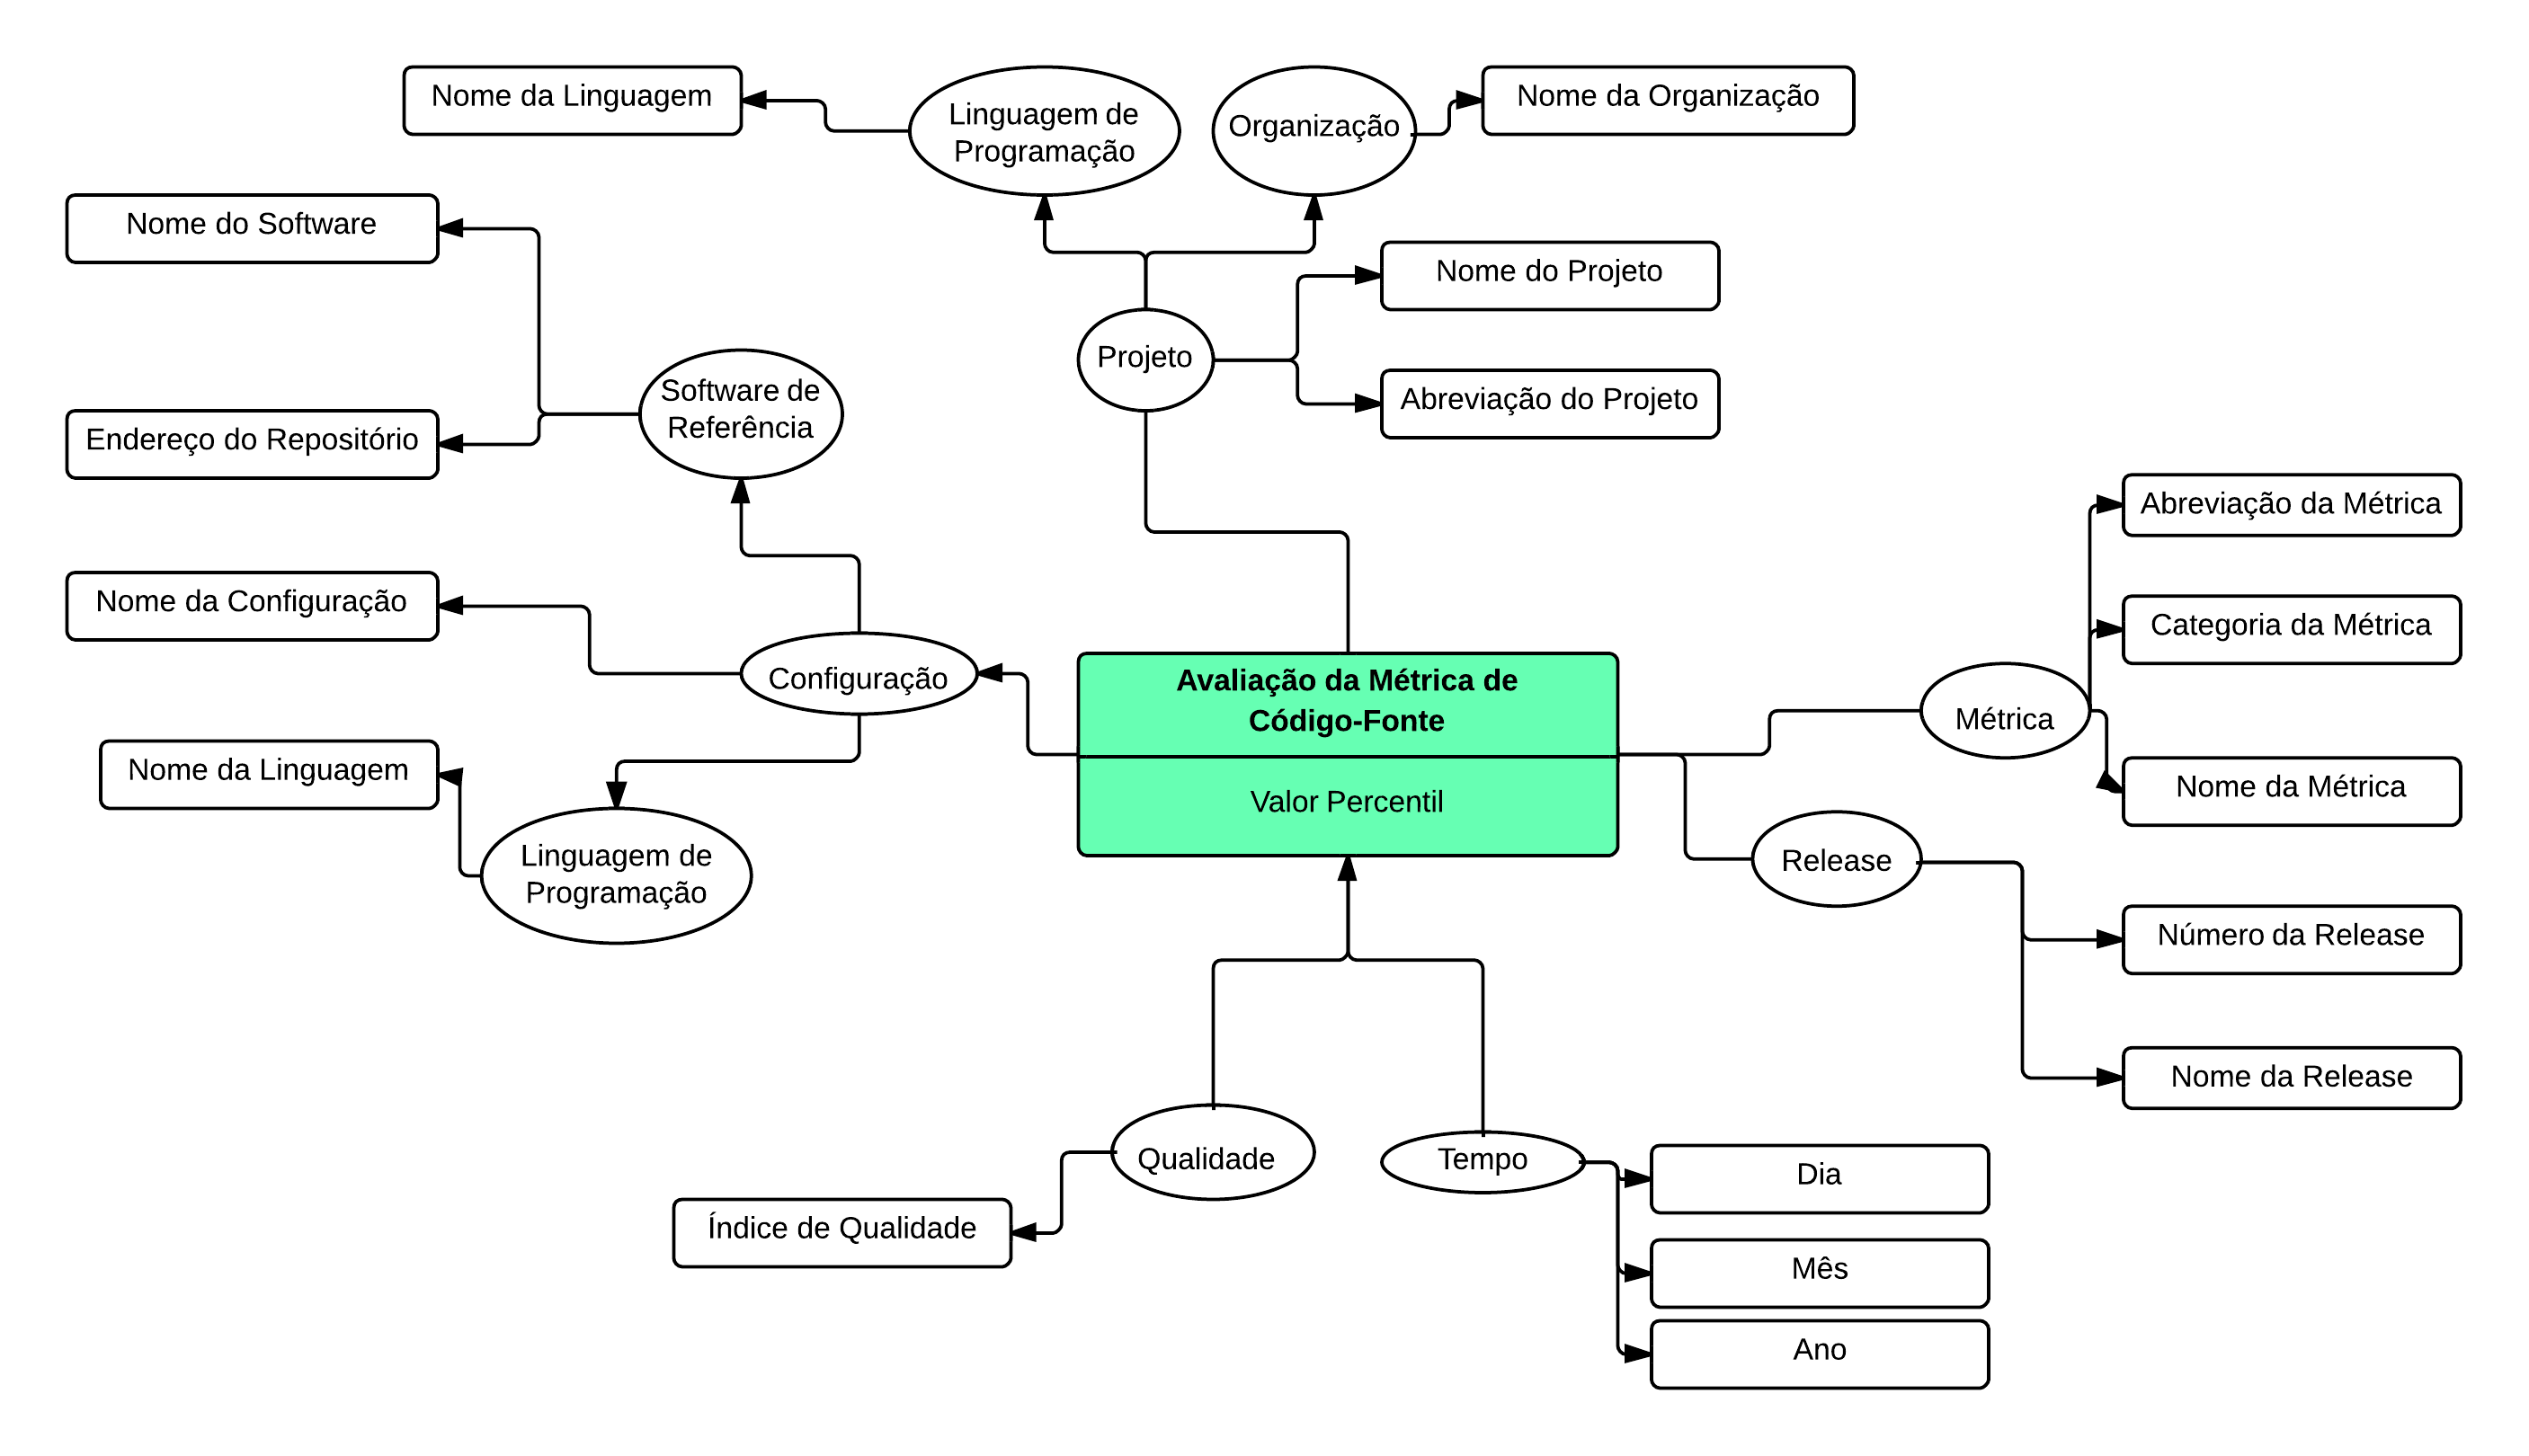
\includegraphics[keepaspectratio=true,scale=0.16]{figuras/percentil-arvore.eps}
\caption{Diagrama de Árvore para Valor Percentil das Métricas de Código-Fonte}
\label{fig:percentil-arvore}
\end{figure}
\FloatBarrier


\begin{figure}[h]
\centering
\includegraphics[keepaspectratio=true,scale=0.20]{figuras/cenario-arvore.eps}
\caption{Diagrama de Árvore para Avaliação de Cenários de Limpeza de Código-Fonte}
\label{fig:cenario-arvore}
\end{figure}
\FloatBarrier


\begin{figure}[ht!]
\centering
\includegraphics[keepaspectratio=true,scale=0.20]{figuras/taxa-arvore.eps}
\caption{Diagrama de Árvore para avaliação da Taxa de Aproveitamento de Oportunidade de Melhoria de Código-Fonte}
\label{fig:taxa-arvore}
\end{figure}
\FloatBarrier


Após a construção dos diagramas de árvore, o projeto físico do \textit{Data Warehouse} foi construído utilizando a ferramenta MySQL Workbench. Como é possivel observar na Figura \ref{fig:project-dw}, cada digrama de árvore foi traduzido para cada tabela fato (tabelas com destaque verde) com as respectivas tabelas dimensões (tabelas com destaque azul)


\begin{figure}[ht!]
\centering
\includegraphics[keepaspectratio=true,scale=0.49]{figuras/modelo-dw.eps}
\caption{Projeto Físico do \textit{Data Warehouse}}
\label{fig:project-dw}
\end{figure}
\FloatBarrier

Visando facilitar o processo de \textit{Extraction-Transformation and Load}, decidiu-se criar uma área de metadados mostrada na Figura \ref{fig:metadados} com intuito de representar os dados sobre os dados dos processos de negócio.

Esta decisão de projeto foi motivada pela recomendação de que os metadados são todas as informações que constituem informações para os dados que farão parte do \textit{Data Warehouse}, sendo que não há uma única forma de fazê-lo para atender as necessidades técnicas e administrativas. Além disso, a principal vantagem de utilização é facilitar a transformação de dados, no processo de ETL \cite{Kimball2002}.


\begin{figure}[ht!]
\centering
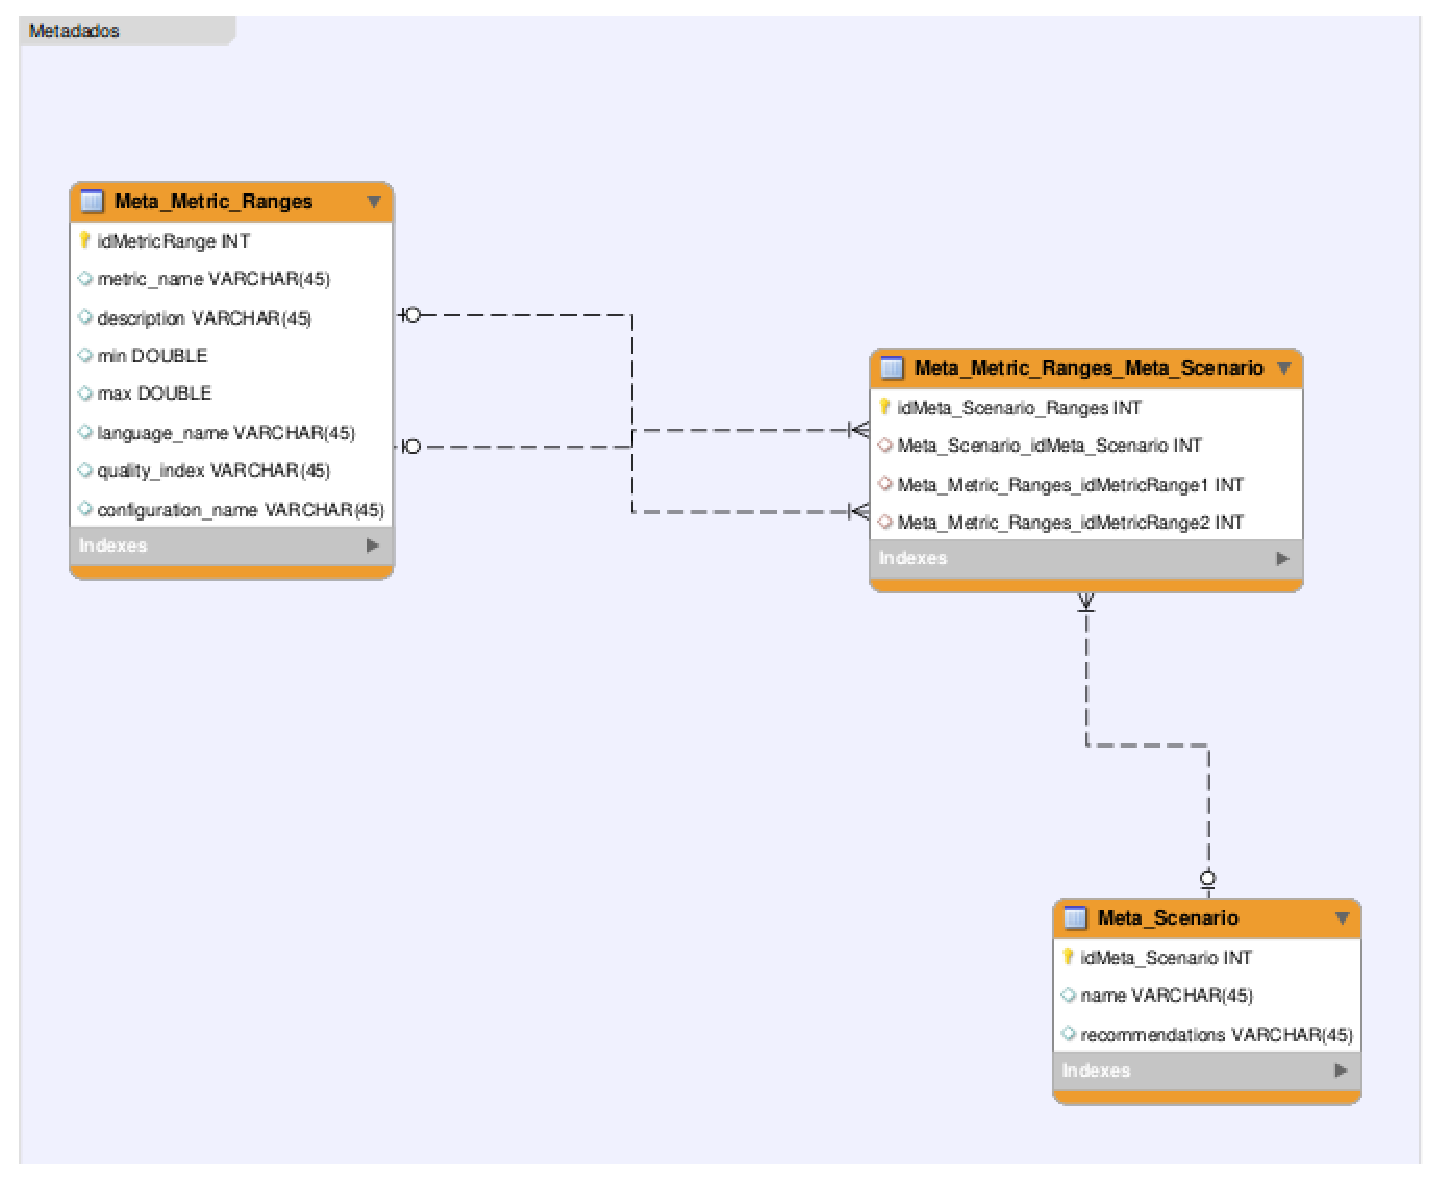
\includegraphics[keepaspectratio=false,scale=0.5]{figuras/metadados.eps}
\caption{Metadados do \textit{Data Warehouse}}
\label{fig:metadados}
\end{figure}
\FloatBarrier


A Tabela~"Meta\_Metric\_Ranges"~contém cada uma das configurações de intervalos qualitativos para cada uma das métricas de código-fonte conforme descrito na Tabela \ref{tab:good-metrics}. Já na Tabela~"Meta\_Scenario"~estão contidos os cenários de limpeza de código-fonte, bem como as recomendações de limpeza para cada um dos cenários conforme descrito na Tabela \ref{tab:cenarios}. 


Para atender o requisito de projeto, observou-se que cada cenário de limpeza identificado é composto por até dois intervalos qualitativos de métricas de código-fonte. Por este motivo, decidiu-se por criar a Tabela~"Meta\_Metric\_Ranges\_Meta\_Scenario"~, com duas chaves estrangeiras da Tabela~"Meta\_Metric\_Ranges", representando as associações entre os cenários de limpeza de código-fonte e os intervalos qualitativos de métricas de código-fonte.



\section{Ferramentas de \textit{Data Warehousing}}

Tendo em vista que o \textit{Data Warehouse} foi projetado em um modelo dimensional, é possível construir tanto o processo de \textit{Extraction-Transformation-Load} quanto as operações de consulta OLAP. Entre as alternativas de código aberto que suportam este ambiente como um todo, está o Pentaho \textit{Business Analytics Community Edition}. Esta solução de software livre apresenta soluções que cobrem 
as áreas de ETL, \textit{reporting}, OLAP e mineração de dados. Cada um dos componentes que foi utilizado é apresentado e analisado nas seções subsequentes.
 


\subsection{Implementação da Extração, Transformação e Carga dos Dados}
\label{implementação-ETL}
O Pentaho \textit{Data Integration Community Edition} ou Kettle \footnote{Disponível em \url{http://kettle.pentaho.com/}} é feito na linguagem Java e implementa o processo de ETL (Extração, Transformação e Carga de Dados). A interface do Kettle é mostrada na Figura \ref{pdi} e as principais características do Kettle bem como a análise quanto aos critérios gerais de seleção de ferramentas são apresentadas na Tabela \ref{kettle}.

\begin{figure}[ht!]
\centering
\includegraphics[keepaspectratio=false,scale=0.38]{figuras/data-integration.eps}
\caption{Interface do Kettle}
\label{pdi}
\end{figure}
\FloatBarrier
 

\begin{table}[!ht]
\input{tabelas/kettle.ltx}
\caption{Características do Kettle e avaliação quanto aos critérios gerais de seleção de ferramentas}
\label{kettle}
\end{table}
\FloatBarrier	

O Kettle possui dois tipos de componentes internos: \textit{Job} e \textit{Transformation}. O primeiro permite executar tarefas, em nível mais alto, de fluxo de controle, tais como, mandar um email em caso de falha, baixar um arquivo, executar transformações  e entre outras atividades. Já a \textit{Transformation} permite tratamento aos dados incluindo desde entrada de dados por diversas fontes até a persistência em uma variedade de SGBDs.


A descrição completa da implementação do processo de \textit{Extraction-Transformation-Load} na ferramenta Kettle foi descrita no Apêndice \ref{sec:implementação-etl}.

\subsection{Implementação das Consultas OLAP e Visualização de Dados}

Para a implementação das consultas OLAP e Visualização de dados, torna-se necessário a utilização do Pentaho BI Platform\footnote{Disponível em \url{http://community.pentaho.com/projects/bi_platform/}}, que é uma ferramenta que provê a arquitetura e a infraestrutura para soluções de \textit{Business Inteligence}, \textit{Data Mining} e a camada de visualização de dados do \textit{Data Warehouse}.


O Pentaho BI Platform, cuja interface inicial é apresentada na Figura \ref{BIplatform}, tem as principais características e a análise quanto aos critérios gerais de seleção de ferramentas são apresentadas na Tabela \ref{biserver}. 


\begin{table}[!ht]
\input{tabelas/biserver.ltx}
\caption{Características do Pentaho BI Platform e avaliação quanto aos critérios gerais de seleção de ferramentas}
\label{biserver}
\end{table}
\FloatBarrier



\begin{figure}[ht!]
\begin{center}
\includegraphics[keepaspectratio=false, scale=0.35]{figuras/bi.eps}
\caption{Interface Gráfica do Pentaho BI Platform}
\label{BIplatform}
\end{center}
\end{figure}
\FloatBarrier
 

A ferramenta Pentaho BI Platform possui arquitetura extensível por plugins diversos que realizam diversas operações, tais como, criação de relatórios, visualização dos dados em tabelas e gráficos e entre outros. Entre os plugins disponíveis, está o Saiku Analytics que oferece serviços de apoio a operações OLAP e à visualização de dados. As características gerais do Saiku Analytics, bem como a avaliação quanto aos critérios gerais de seleção de ferramentas, são apresentados na Tabela \ref{saiku}. 

\begin{table}[!ht]
\input{tabelas/saiku.ltx}
\caption{Características do Saiku Analytics e avaliação quanto aos critérios gerais de seleção de ferramentas}
\label{saiku}
\end{table}
\FloatBarrier

Na arquitetura do Saiku Analytics, está incorporado outro software livre chamado de Mondrian OLAP. Por meio dele, é possível realizar  consultas. Estas ocorrem por meio da escrita de \textit{queries} em linguagem MDX \textit{(MulitDimensional eXpressions)}, que foi proposta por \citeonline{spofford2006mdx} como uma forma de escrever consultas mais otimizadas para bases que seguem o modelo dimensional, tal como mostra o exemplo do trecho de Código-Fonte \ref{MDX}.


\begin{center}
\begin{minipage}{0.5\textwidth}

\begin{lstlisting}[caption=Exemplo de \textit{Query} em linguagem MDX, label=MDX]
 SELECT
   { [Measures].[Loja] } ON COLUMNS,
   { [Tempo].[2002], [Tempo].[2003] } ON ROWS
FROM Vendas
WHERE ( [Loja].[Loja Sul]) 

\end{lstlisting}
\end{minipage}
\end{center}
\FloatBarrier

\newpage
\section{Resumo das Ferramentas utilizadas do Ambiente de \textit{Data Warehousing}}

Na Figura \ref{pentaho-tools}, é apresentado o modo como cada uma das ferramentas apresentadas na seções anteriores está disposta na arquitetura do ambiente de \textit{Data Warehousing} para Métricas de Código-Fonte.

\begin{figure}[ht!]
\begin{center}
\includegraphics[keepaspectratio=true, scale=.20]{figuras/pentaho-tools.eps}
\caption{Arquitetura Ambiente de \textit{Data Warehousing} para Métricas de Código-Fonte}
\label{pentaho-tools}
\end{center}
\end{figure}
\FloatBarrier

A arquitetura descrita na Figura \ref{pentaho-tools} foi implementada em uma máquina virtual com as seguintes configurações:

\begin{easylist}
& Processador: Intel(R) Xeon(R) CPU E5-2620 @ 2.00GHz
& RAM: 8GB
& Distribuição: Debian Whezzy
\end{easylist}